\documentclass{beamer} 
\usetheme{metropolis}
% \usecolortheme{spruce}
\decimalpoint
\setlength{\parindent}{0cm}
\usepackage{color}
\usepackage[utf8]{inputenc}
\usepackage[spanish]{babel}
\usepackage{amsmath}
\usepackage{amsfonts}
\usepackage{amssymb}
\usepackage{graphicx}
\usepackage{ragged2e}
\usepackage{caption}
\usepackage{subcaption}
\usepackage{tikz}
\usepackage{tcolorbox}
\usepackage{float}
\usepackage{epigraph}
\usepackage{fontawesome}
\usepackage{array}
\newcolumntype{P}[1]{>{\centering\arraybackslash}p{#1}}


\newtcolorbox{informacion}[2][]
{
  breakable,
  colframe = blue!5!white,
  colback  = blue!5!white,
  coltitle = blue!80!black,
  title    = \faInfo \hspace{5 mm} #2,
}

\newtcolorbox{ejemplo}[2][]
{
  breakable,
  colframe = gray!50,
  colback  = gray!0,
  coltitle = gray!20!black,
  title    =  \faEdit \hspace{5 mm} #2,
}



\title{
{\Large Mecánica de Materiales} \\
{\large I. Esfuerzo y deformación}
}
\author{Pedro Jorge De Los Santos}
\institute{
    {\bf 
    Instituto Tecnológico de Celaya \\
    Departamento de Ingeniería Mecánica \\
    }
}

\apptocmd{\frame}{}{\justifying}{}
\begin{document}

\begin{frame}
\titlepage
\end{frame}

% Sección introducción
\section{Introducción a la mecánica de materiales}

\begin{frame}
\justifying
\frametitle{Introducción a la mecánica de materiales}


La mecánica de materiales \footnote{También conocida como Resistencia de Materiales} es una rama de la 
mecánica aplicada que estudia el comportamiento de cuerpos sólidos sometidos a diversas cargas, incluyendo 
en esta definición a todo tipo de elementos estructurales: barras, columnas, vigas, armaduras, ejes; sometidos a 
diversas configuraciones de carga: axiales, a torsión, compresión y/o una combinación de las anteriores. \\

El objetivo principal de la mecánica de materiales es determinar los esfuerzos, las deformaciones 
unitarias y los desplazamientos en estructuras y sus componentes debidas a las cargas que actúan sobre 
ellas. \\

\end{frame}


\begin{frame}
\frametitle{Esfuerzo en una estructura}
\justifying

Los conceptos fundamentales de esfuerzo y deformación pueden ser ilustrados considerando una barra 
prismática cargada axialmente con una fuerza P en sus extremos.  La fuerza axial 
produce un estrechamiento uniforme en la barra, en este caso se dice que la barra está a tensión. \\

\hfill \\

\begin{informacion}{Barra prismática}
Una barra prismática es un elemento 
estructural recto que tiene una misma sección transversal a lo largo de su longitud.
\end{informacion}

\end{frame}


\begin{frame}
\frametitle{Esfuerzo en una estructura}
\justifying

La fuerza por unidad de área, o intensidad de las fuerzas distribuidas sobre una sección dada, es 
llamada esfuerzo en esa sección y se denota con la letra griega $\sigma$ y viene dado por:

\begin{equation}\label{eq:esfuerzo}
\sigma = \frac{P}{A}
\end{equation}

\begin{center}
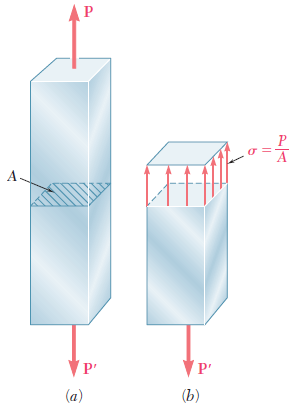
\includegraphics[width=0.3\textwidth]{img/axial_load.PNG}
\end{center}

\end{frame}


\begin{frame}
\frametitle{Esfuerzo en una estructura}
\justifying

Las unidades usuales para cada magnitud involucrada en la ecuación \ref{eq:esfuerzo} se resumen en 
la siguiente tabla:

\begin{table}[h!]
\centering
% \rowcolors{1}{}{gray!20}
\begin{tabular}{P{3cm} P{3cm} P{3cm}}
\hline
\bfseries Magnitud & \bfseries SI & \bfseries Sistema Inglés \\
\hline
P (Fuerza) & N & lb \\
A (Área) & $m^2$ & $in^2$ \\
$\sigma$ (Esfuerzo) & Pa & psi \\
\hline
\end{tabular}
% \caption{Valores especiales}
\end{table}

\begin{informacion}{Convención de signos}
Se utiliza un signo positivo para indicar un esfuerzo de tensión y un signo negativo para especificar un 
esfuerzo de compresión.
\end{informacion}



\end{frame}








\begin{frame}
\frametitle{Ejemplos}
\justifying

\begin{ejemplo}{Ejemplo 1}

Una barra prismática con sección transversal rectangular como se muestra en la figura, está sujeta a 
una carga axial a tensión $P$. La elongación medida en la barra es de $\delta = 1.2 \,\, \text{mm}$. 
Calcular el esfuerzo normal y la deformación unitaria en la barra, sabiendo que $L = 3\,\text{m} $, 
$P = 50 \, \text{kN}$, $a=20 \, \text{mm}$ y $b=40 \, \text{mm}$.

\begin{center}
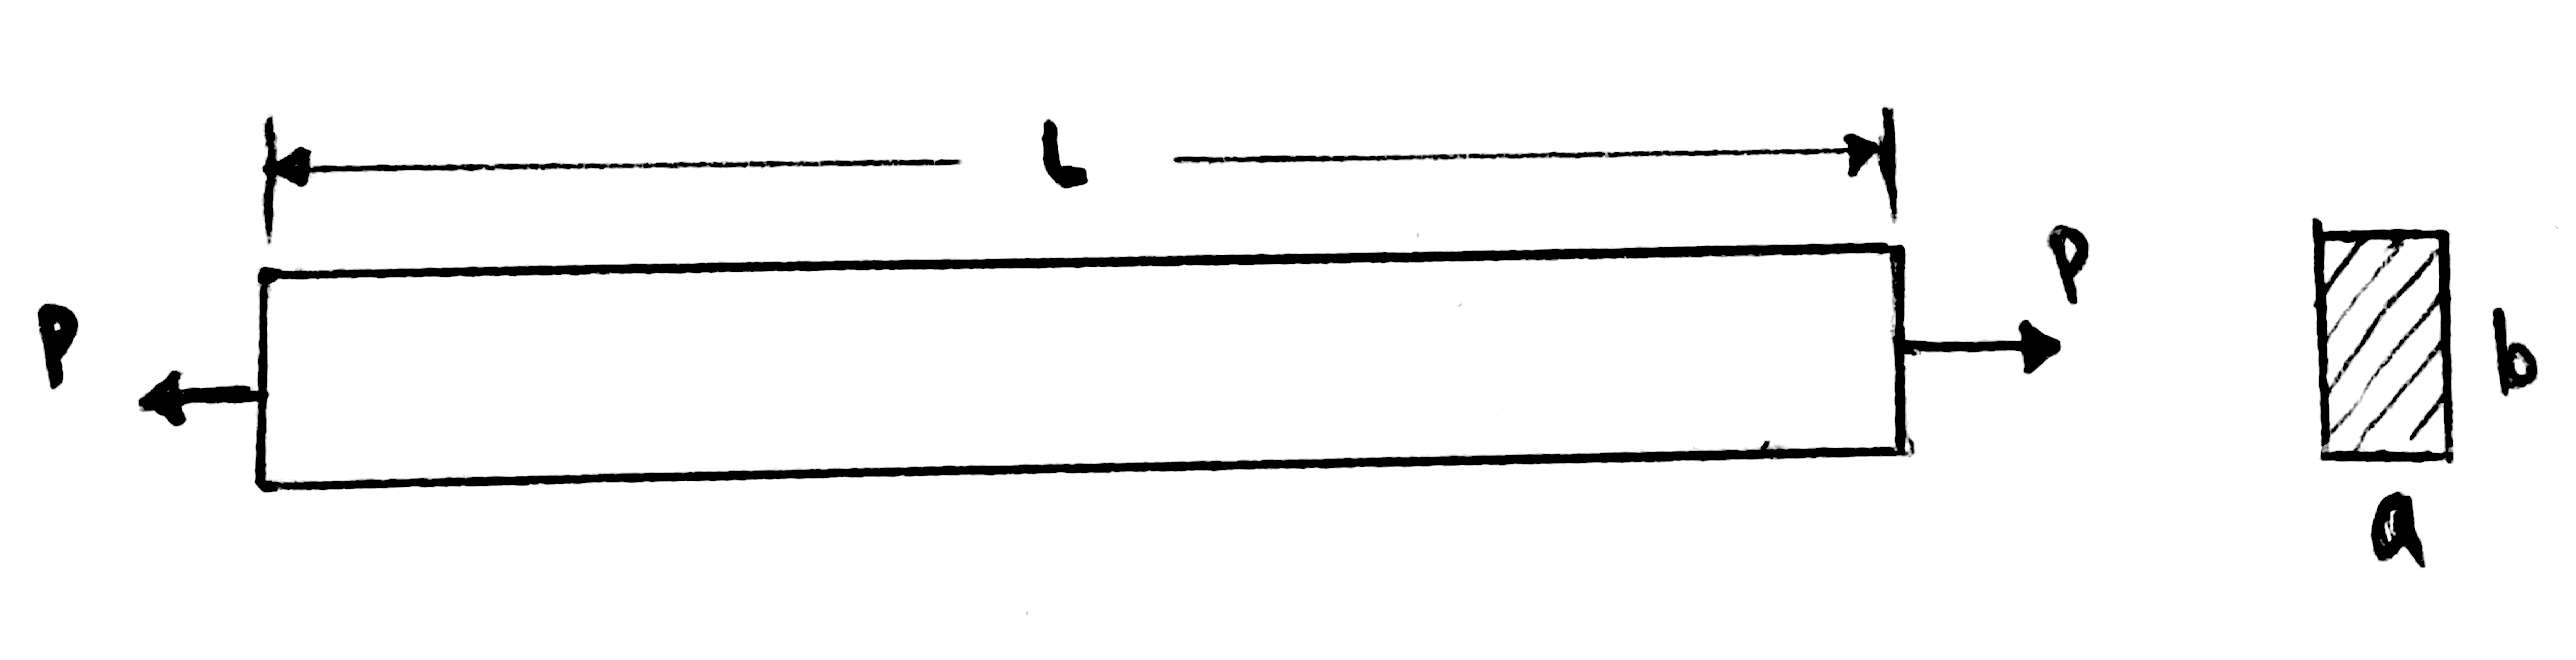
\includegraphics[width=0.55\textwidth]{img/ejemplo_01.jpg}
% \captionof{figure}{Barra prismática sometida a tensión}
% \label{fig:barra_tension}
\end{center}

Calculando el esfuerzo, se tiene:

$$ \sigma = \frac{P}{A} = \frac{50 000}{(0.02)(0.04)} = 62.5 \, \text{MPa} $$
\end{ejemplo}

\end{frame}


\begin{frame}

\begin{ejemplo}{}
Para la deformación unitaria:

$$ \epsilon = \frac{\delta}{L} = \frac{0.0012}{3} = 400 \mu $$

De lo anterior, hay que poner atención sobre las unidades en las cuales estamos trabajando, 
para obtener resultados coherentes en unidades consistentes.
\end{ejemplo}


\end{frame}


\begin{frame}
\frametitle{Referencias}

\begin{enumerate}
\item Beer, F. P. (2013). Mecánica de materiales. México, D.F: McGraw-Hill Interamericana.
\item Gere, J. M., Goodno, B. J., & León, C. J. (2014). Mecánica de materiales. Australia: Thomson Learning.
\item Gere, J., & Timoshenko, S. (1998). Mecǹica de materiales. Mx̌ico, D.F: Thomson Learning.
\item Hibbeler, R. C., Murrieta, M. J. E., Molina, S. O., & Saldaña, S. S. (2011). Mecánica de materiales. Naucalpan de Juárez, México: Pearson educación.
\end{enumerate}
\end{frame}

\begin{frame}
\justifying
\frametitle{...}

El contenido de esta presentación está basado en las referencias bibliográficas básicas del curso. 
Si no se indica de manera explícita, las imágenes y diagramas corresponden a la referencia [1].

\end{frame}


\end{document}

